\documentclass[10pt]{article}

\usepackage{graphicx}
\usepackage{float}
\usepackage{subcaption}
\usepackage{amsmath}
\usepackage{amssymb}
\usepackage{multicol}
\usepackage[a4paper,margin=0.75in,footskip=0.25in]{geometry}
\graphicspath{{Images/}}

%\addtolength{\oddsidemargin}{-1.5in}
%\addtolength{\evensidemargin}{-1.5in}
%\addtolength{\textwidth}{1.75in}
%\addtolength{\topmargin}{-.7in}
%\addtolength{\textheight}{1.75in}



\setlength{\columnsep}{1cm}

\numberwithin{equation}{section}

\begin{document}
\author{ David Strachan and Edward Gandar }
\title{\textbf{Stability of a dipolar BEC in a pancake potential using the Dini expansion Hankel transform}}

\maketitle

\tableofcontents

\pagebreak

\begin{multicols}{2}

\section{The Gross-Pitaevskii equation (GPE) for dipolar condensates in three dimensions}

At ultra-low temperatures the properties of a dipolar condensate with $N$ atoms, each of mass $m$, can be described by the GPE below.

\begin{multline}
i\hbar \frac{\partial \psi(\textbf{r},t)}{\partial t}=\bigg[-\frac{\hbar^2}{2m}\nabla^2 + V_{ext}(\textbf{r}) + \frac{4\pi \hbar^2 a_{s} N}{m}|\psi(\textbf{r}',t)|^2 \\+ N \int_V U_{dd}(\textbf{r}-\textbf{r}')|\psi(\textbf{r},t)|^2d^3\textbf{r}' \bigg]\psi(\textbf{r},t)
\end{multline}

where $\int_V d^3\textbf{r} |\psi(\textbf{r},t)|^2 = 1$ and $a_{s}$ is the atomic s-wave scattering length. The trapping potential is assumed to be either in the form $$V_{ext}=\frac{1}{2}m(w^2 x^2+w^2 y^2+w_{z}^2z^2)$$ and is assumed to have cylindrical symmetry about the z axis, or a circle box potential of radius R,
\begin{equation*}
V_{ext}(r) = 
\begin{cases}
0 & \text{for $r<R$} \\
\infty & \text{otherwise}
\end{cases}
\end{equation*}

and $$V_{ext}(z)=\frac{1}{2}mw_{z}^2z^2$$ harmonic in the z axis. Where $w$ is the angular frequency.

The dipolar interaction, for magnetic dipoles, is described by the equation:
\begin{equation}
U_{dd}(\textbf{r}-\textbf{r}') = \frac{\mu_{0} \bar{\mu}^2}{4\pi} \frac{1-3 \cos^2{(\theta)}}{|\textbf{r}-\textbf{r}'|^3}
\end{equation}
where $\theta$ is the angle between $\textbf{r}-\textbf{r}'$ and the direction of the polarization (chosen to be z) $\mu_{0}$ is the permeability of free space, and $\bar{\mu}$ is the dipole moment of the atom.

In the case of the harmonic potential, we go into dimensionless units: $t \mapsto t_s t, \textbf{r} \mapsto x_s\textbf{r}$, $\psi \mapsto \ \psi x_{s}^{-\frac{3}{2}}$, with $x_{s}=\sqrt{\frac{\hbar}{m\omega}}$ and $t_s=\omega = \text{min}(w_x,w_y,w_z)$ we end up with the equation
\begin{multline}
i\frac{\partial \psi(\textbf{r},t)}{\partial t}=\bigg[-\frac{1}{2}\nabla^2 + V_{trap} + g_{s}|\psi(\textbf{r},t)|^2 \\+ D \int_V U_{3D}(\textbf{r}-\textbf{r}')|\psi(\textbf{r}',t)|^2 d^3\textbf{r}' \bigg]\psi(\textbf{r},t)
\end{multline}

where
\begin{equation}
V_{trap}=\frac{1}{2}(\gamma_{x}^2 x^2+\gamma_{y}^2 y^2+\gamma_{z}^2 z^2)
\end{equation}
and
\begin{equation}
U_{3D}(\textbf{r}-\textbf{r}')=\frac{1-3 \cos^2{(\theta)}}{|\textbf{r}-\textbf{r}'|^3}
\end{equation}

where \scalebox{1.2}{$g_{s}=\frac{4 \pi a_{s} N}{x_s}$}, \scalebox{1.2}{$\gamma_{i}=\frac{w_{i}}{w}$, $i=x,y,z$}, is the trap ratio and \scalebox{1.2}{$D=\frac{m N \mu_{0} \bar{\mu}^2}{4 \pi \hbar^2 x_s}$}.

Similarly in the case of the box potential, we go into dimensionless units, however the natural length and time scales are different Refs \cite{Bao_2013},\cite{Galati_2013},\cite{Oganesov_2018}. Namely, $x_s=L$ where $L$ is a chosen fraction of the size (radius) of the box, and \scalebox{1.1}{$t_s = \frac{mL^2}{\hbar}$}. We thus end up with the equation
\begin{multline}
i\frac{\partial \psi(\textbf{r},t)}{\partial t}=\bigg[-\frac{1}{2}\nabla^2 + V_{trap} + g_{s}^{box}|\psi(\textbf{r},t)|^2 \\+ D^{box} \int_V U_{3D}(\textbf{r}-\textbf{r}')|\psi(\textbf{r}',t)|^2 d^3\textbf{r}' \bigg]\psi(\textbf{r},t)
\end{multline}
where
\begin{equation*}
V_{trap}(r) = 
\begin{cases}
0 & \text{for $r<\alpha$} \\
\infty & \text{otherwise}
\end{cases}
\end{equation*}

and
\begin{equation}
V_{trap}(z)=\frac{1}{2} \frac{m^2w_{z}^2 L^4}{\hbar^2}z^2 \label{Vextbox}
\end{equation}
 harmonic in the z axis.

where \scalebox{1.2}{$g_{s}^{box} = \frac{4 \pi N a_s}{L}$}, \scalebox{1.2}{$D^{box} =  \frac{m N \mu_0 \bar{\mu}^2}{4\pi \hbar^2 L}$}
and \scalebox{1.2}{$\alpha = \frac{R_{box}}{L}$}. The reason for doing this instead of simply having  \scalebox{1.2}{$R_{box} = L$}, where $R_{box}$ is 
the radius if the trap is explained in section [INSERT SECTION NAME].

PLEASE CHECK IF THIS IS VALID


\section{Evaluation of dipole interaction}
The long-range anisotropic dipole potential is usually hard to calculate, however the integral is efficiently evaluated in Fourier space with the use of the convolution theorem Ref\cite{bland2018elementary}. Recall the dipolar interaction term $\Phi_{dd}(\textbf{r},t)$, stated again here as:
\begin{equation}
\Phi_{dd}(\textbf{r},t) = \int_V d^3\textbf{r}' U_{dd}(\textbf{r}-\textbf{r}')|\psi(\textbf{r}',t)|^2
\end{equation}
The convolution theorem allows us to rewrite this as
\begin{equation}
\Phi_{dd}(\textbf{r},t) = \mathcal{F}^{-1} [ \tilde{U_{dd}}(\textbf{k})\tilde{n}(\textbf{k},t)]
\end{equation}

where $\mathcal{F}$ ($\mathcal{F}^-1$) denotes the (inverse) Fourier transform, $\tilde{U_{dd}}(\textbf{k}) = \mathcal{F}[U_{dd}(\textbf{r})]$ is the k-space dipolar potential, and $\tilde{n}(\textbf{k},t)$ is the density in k-space. The numerical calculation of this convolution is simply handled by the fast Fourier transforms (FFT) algorithms. However, since the FFT algorithms are naturally periodic, alias copies of the system can interact, by virtue of the long-range nature of the dipole interaction. In order to overcome this effect, we assume cylindrical symmetry of the system, which allows us to make use of a Hankel transform which does not assume periodicity, and thus doesn't produce alias copies. This also has the added benefit of reducing the number of effective dimensions from 3D (x,y,z), to 2D (r,z), which also greatly reduces computational time. (We will discuss this more in detail later in section 3). We also truncate the dipole potential in the z direciton to ensure that phantom copies cannot interact.

If the hankel transform is not used the standard truncated forms of the dipole term are the following. The first variant involves a spherical cut-off, which is used for almost-spherical sized systems (small $\gamma_i$). Restricting the range of the dipole interaction to a sphere of radius $R_c$, gives us the potential

\begin{equation}
U_{dd}^{R_c}(\textbf{r}-\textbf{r}') = 
\begin{cases}
\frac{\mu_{0} \bar{\mu}^2}{4\pi} \frac{1-3 \cos^2{(\theta)}}{|\textbf{r}-\textbf{r}'|^3}, & \text{for $r<R_c$} \\
0, & \text{otherwise}
\end{cases}
\end{equation}
As long as $R_c > R_{max}$ where $R_{max}$ is the system size, this potential should reduce the effect of alias copies. The analytical Fourier transform is
 
\begin{equation}
\tilde{U_{dd}}(k) = \frac{C_{dd}}{3}\bigg[1+3\frac{\cos(R_{c}k)}{(R_{c}k)^{2}}-3\frac{\sin(R_{c}k)}{(R_{c}k)^{3}}\bigg](3\cos{(\theta_{k})^2}-1)
\end{equation}

This works for near-spherical traps, but if the system is highly oblate (if the trap is pancake like), the grid size in each dimension must still extend beyond $R_{max}$. This means the number of grid points in the tight direction required must be large to ensure sufficient resolution. A fix to this problem is to introduce a cylindrical cut-off to the dipole potential, given as

\begin{equation}
U_{dd}^{R_c}(\textbf{r}-\textbf{r}') = 
\begin{cases}
\frac{\mu_{0} \bar{\mu}^2}{4\pi} \frac{1-3 \cos^2{(\theta)}}{|\textbf{r}-\textbf{r}'|^3}, & \text{for $\rho<\rho_c$ and $|z|<Z_c$} \\
0, & \text{otherwise}
\end{cases}
\end{equation}

The Fourier transform is semi-analytic \cite{bland2018elementary}
\begin{multline}
\tilde{U_{dd}}(\textbf{k}) = \frac{C_{dd}}{3}(3\cos{\theta_k}^{2}-1) \\+ C_{dd}e^{-Z_{c}k_{\rho}}[\sin{\theta_{k}}^{2}\cos{Z_{c}k_{z}} -\sin{\theta_{k}}\cos{\theta_{k}}\sin{Z_{c}k_{z}}] \\- C_{dd}\int_{\rho_{c}}^{\infty}\rho d\rho\int_{0}^{Z_{c}}dz\cos{k_{z}z}\frac{\rho^{2}-2z^{2}}{(\rho^{2}+z^{2})^{\frac{5}{2}}}J_{0}(k_{\rho}\rho),
\end{multline} 
Where $J_{0}$ is the zeroth order Bessel function of the first kind.

The final line cannot be done analytically, but requires numerical integration, which is computationally costly but only required once per simulation set-up. However, if the integral is not calculated, the first two terms act as a dipole interaction truncated in the z direction only Ref\cite{Ronen_2006}. We use this form of the dipole potential, since the use of the Hankel transform in the $\rho$ direction does not produce alias copies and thus does not need to be truncated. The Hankel transform is discussed in more detail in the next section.

\section{Hankel Transform using the Dini expansion}
If the dipole polarization is along the z axis, the ground state will be cylindrically symmetric in a harmonic trap (or circular box potential). This can reduce a 3D system to an effective 2D system, where only the r and z coordinates are needed. If we are in cylindrical coordinates, the space where the r component of the Laplacian operator is diagonalised is bessel space (more specifically zeroth order bessel functions of the first kind). To transform from position space to bessel space, we use a Hankel transform. In ref \cite{Kai_Ming_2009} they outline a very efficient method to compute a discrete Hankel transform for a finite range of r. 
First, we rewrite the function in both position space $f(r)$ and bessel space $g(\rho)$ as a Dini series. 



If $0<r<b$ and $0<\rho<\beta$ then we can write f(r) and $g(\rho)$ as
\begin{equation}
f(r) = \frac{2}{b^{2}}\sum_{n=0}^{\infty}f_{n}J_{0}^{-2}(\alpha_{n})J_{0}(\frac{\alpha_{n}r}{b})
\end{equation}
\begin{equation}
g(\rho) = \frac{2}{\beta^{2}}\sum_{n=0}^{\infty}g_{n}J_{0}^{-2}(\alpha_{n})J_{0}(\frac{\alpha_{n}\rho}{\beta})
\end{equation}
where 
\begin{equation}
f_{n} = \int_{0}^{b}rf(r)J_{0}(\frac{\alpha_{n}r}{b})dr=\frac{1}{2\pi}g(\frac{\alpha_{n}}{2\pi b})
\end{equation}
and
\begin{equation}
g_{n} = \int_{0}^{\beta}\rho g(\rho)J_{0}(\frac{\alpha_{n}\rho}{\beta})d\rho=\frac{1}{2\pi}f(\frac{\alpha_{n}}{2\pi\beta})
\end{equation}
where $\alpha_{n}$ are the real nonnegative roots of the derivative of the zero-order Bessel function, $\alpha_{0}=0$. We can truncate these infinite sums to finite ones by using the fact that if $\alpha_{N} >S$ where $S=2\pi b\beta$, both $f_{N}$ and $g_{N}$ are zero.

Defining a change of variables, 
\begin{equation}
G(m) = g(\frac{\alpha_{m}}{2\pi b})|J_{0}^{-1}(\alpha_{m})|\beta
\end{equation}
\begin{equation}
F(n) = f(\frac{\alpha_{n}}{2\pi \beta})|J_{0}^{-1}(\alpha_{n})|b
\end{equation}
leads to the following formula for the discrete Hankel transform and its inverse,
\begin{equation}
G(m) = \sum_{n=0}^{N}c_{mn}F(n)
\end{equation}
\begin{equation}
F(n) =  \sum_{m=0}^{N}c_{nm}G(m)
\end{equation}
where $c_{nm}$ are the elements of a transform matrix, 
\begin{equation}
c_{nm} = \frac{2}{S}|J_{0}^{-1}(\alpha_{n})||J_{0}^{-1}(\alpha_{m})|J_{0}(\frac{\alpha_{n}\alpha_{m}}{S})
\end{equation}
For this to hold, the matrix C has to satisfy $CC =I$, and C is a function of S only so S must be chosen correctly. In \cite{Kai_Ming_2009} they state that the optimum choice is 
\begin{equation}
S = 2|J_{0}^{-1}(\alpha_{k})|\sqrt(1+\sum_{n=1}^{N}J_{0}^{-2}(\alpha_{n})J_{0}^{2}(\frac{\alpha_{k}\alpha_{n}}{J_{N+1}}))
\end{equation}
where 
\begin{equation}
k = Int(\frac{N}{4})
\end{equation}
Despite redefining S in a different way, as long as $S<\alpha_{N+1}$, this approach is still valid.
 
  Further efficiency can be achieved by realising all solutions will be symmetric in z, so only $z\geqslant0$ is needed. Instead of using a Fourier transform we can use a fast cosine transform, which leads to faster computational time overall.
  
\section{Extending the Hankel Transform to the non-symmetric case}

I'll outline this separately to the symmetric case, but it's just the general case so includes the above transform that we use for the code. 
\\
It isn't only the fact it can reduce the dimensions of the problem that makes the Hankel transform useful, but it needs no assumption of periodicity unlike the fourier transform, meaning no cut off is needed. The reason for this being such an advantage is that the integral in Eq 2.6 is quite computationally costly, and depends on various parameters meaning this integral may have to be repeatedly calculated if any of these parameters change. So, even in the non-symmetric case, an extension to the method outlined in ref \cite{Kai_Ming_2009} which doesn't assume symmetry would be very useful.
The Dini series is based on the Robin boundary condition where if the following is true,

\begin{equation}
 bf'(b) +c_{r}f(b)=0, 
\end{equation}
where $c_{r}$ is a constant, then a function f(r) defined for $r\geqslant0$ can be expressed as 
\begin{equation}
f(r) = \frac{2}{b^{2}}\sum_{n=0}^{\infty}f_{n}J_{\nu}^{-2}(\lambda_{\nu,n})J_{\nu}(\lambda_{\nu,n}r/b)
\end{equation}
where $\lambda_{\nu,n}$ is the nth root of 
\begin{equation}
rJ'_{\nu}(r)+c_{r,\rho}J_{\nu}(r)=0.
\end{equation}
The coefficients $f_{n}$ are given by
\begin{multline}
f_{n} = \frac{\lambda^{2}_{\nu,n}}{c^{2}_{r}+\lambda^{2}_{\nu,n}-\nu^{2}} \int_{0}^{b}rf(r)J_{\nu}(\lambda_{\nu,n}r/b)dr \\= \frac{\lambda^{2}_{\nu,n}}{2\pi(c^{2}_{r}+\lambda^{2}_{\nu,n}-\nu^{2})} \mathcal{F}_{\nu}(\lambda_{\nu,n}/2\pi b)
\end{multline}
 $\mathcal{F}_{\nu}(\rho)$ represents the function f(r) in $\nu^{th}$ order bessel space. As this is also defined for  $\rho\geqslant0$, the following is also true
\begin{equation}
\mathcal{F}_{\nu}(\rho)= \frac{2}{\beta_{\nu}^{2}}\sum_{n=0}^{\infty}g_{n}J_{\nu}^{-2}(\lambda_{\nu,n})J_{\nu}(\lambda_{\nu,n}\rho/\beta_{\nu})
\end{equation}
given 
\begin{equation}
\beta_{\nu}\mathcal{F}'_{\nu}(\beta_{\nu})+c_{\rho}\mathcal{F}_{\nu}(\beta_{\nu})=0, 
\end{equation}
The coefficients $g_{n}$ are given by
\begin{multline}
g_{n} = \frac{\lambda^{2}_{\nu,n}}{c^{2}_{\rho}+\lambda^{2}_{\nu,n}-\nu^{2}} \int_{0}^{\beta_{\nu}}\rho\mathcal{F}_{\nu}(\rho)J_{\nu}(\lambda_{\nu,n}\rho/\beta_{\nu})d\rho \\= \frac{\lambda^{2}_{\nu,n}}{2\pi(c^{2}_{\rho}+\lambda^{2}_{\nu,n}-\nu^{2})}f(\lambda_{\nu,n}/2\pi\beta_{\nu})
\end{multline}
Technically $\lambda_{\nu,n}$ has to be defined differently for (4.5) and (4.7) if $c_{\rho} \neq c_{r}$, but as we will see this is never the case.
There are two main differences in the structure of this for a general $\nu\in\mathbb{Z}^{+}$ compared to the $\nu=0$ case. The first and main problem is the potential for asymptotes if 
\begin{equation}
c^{2}_{r,\rho}+\lambda^{2}_{\nu,n}=\nu^{2}, 
\end{equation}
bearing mind that $\lambda_{\nu,n}$ takes many values and there is nothing preventing Eq 4.8 being true. We can easily get past this by realising that the choice of $c_{r,\rho}$ is arbitary. $c_{r,\rho}$ is(are) based on the Robin boundary condition, and because our system is bounded, 
\begin{equation}
f(r\geqslant b) = 0
\end{equation}
\begin{equation}
\mathcal{F}_{\nu}(\rho\geqslant\beta_{\nu}) = 0.
\end{equation}
Then, the only condition for (4.1) and (4.6) to hold is
\begin{equation}
 \mathcal{F}'_{\nu}(\beta_{\nu}) = 0 = f'(b).
\end{equation}
and this is independent of $c_{r,\rho}$. The validity of (4.11) comes from the fact that as $f(x)\Rightarrow0$, $f'(x)\Rightarrow0$ provided both of these are smooth and continuous. I'm pretty sure this is true, otherwise the probability current would be non zero at the boundary so probability wouldn't be conserved. If, for any given $\nu$ we set $c_{r}=c_{\rho}=\nu$ this asymptotic behaviour no longer appears. This also leads to a simplifed expression as $\lambda^{2}_{\nu,n}$ cancels. This choice leads to the second difference, which is the nature of the roots $\lambda_{\nu,n}$. Inserting this value of c into Eq (4.3) leads to
\begin{equation}
rJ'_{\nu}(r)+\nu J_{\nu}(r)=0.
\end{equation}
($c = -\nu$ also works, which might cause problems if it leads to different solutions, I haven't checked this).
Using the following recurrence relations for Bessel functions,
\begin{equation}
J_{\nu-1}(z)-J_{\nu+1}(z) = 2J'_{\nu}(z),
\end{equation}
\begin{equation}
J_{\nu-1}(z)+J_{\nu+1}(z) = \frac{2\nu}{z}J_{\nu}(z),
\end{equation}
Eq (4.12) simplifies to 
\begin{equation}
2\nu J'_{\nu}(r)-rJ_{\nu-1}(r)=0.
\end{equation}
This has to be solved numerically, but it's essentially equating two Bessel functions of adjacent order so we could write a function which takes the two bessel functions as arrays (with the $2\nu$ and r prefactors) and then takes one away from the other. The output would be an array of the r values when they're equal, which probably doesn't take long at all. Further to this, for a given $\nu$ this only has to be calculated once as it doesn't depend on any parameters of our system apart from the number of data points in our r array, which will be the number of roots we need. But again, a large number $N_{max}$ can be calculated so even if N is changed, provided $N<N_{max}$ the roots won't have to be recalculated.

\subsection{The Form of the General Hankel Transform}

If $\lambda_{\nu,N}>S$ where $S_{\nu}=2\pi b\beta_{\nu}$, both $f_{n}$ and  $g_{n}$ are zero for $n\geqslant\ N$. Defining a change of variables, (I realise this notation is poor because I've already used $\mathcal{F}_{\nu}$ to define f in bessel space, I can change this)
\begin{equation}
G_{\nu}(m) = \mathcal{F}_{\nu}(\frac{\lambda_{\nu,m}}{2\pi b})|J_{\nu}^{-1}(\lambda_{\nu,m})|\beta_{\nu}
\end{equation}
\begin{equation}
F_{\nu}(n) = f(\frac{\lambda_{\nu,n}}{2\pi \beta_{\nu}})|J_{\nu}^{-1}(\lambda_{\nu,n})|b
\end{equation}
leads to the formula for the general, discrete Hankel transform and its inverse for any $\nu\in\mathbb{Z}^{+}$,
\begin{equation}
G_{\nu}(m) = \sum_{n=0}^{N}C_{\nu,mn}F_{\nu}(n)
\end{equation}
\begin{equation}
F_{\nu}(n) =  \sum_{n=0}^{N}C_{\nu,nm}G_{\nu}(m)
\end{equation}
where $C_{\nu,nm}$ are the elements of a transform matrix, 
\begin{equation}
C_{\nu,nm} = \frac{2}{S_\nu}|J_{\nu}^{-1}(\lambda_{\nu,n})||J_{\nu}^{-1}(\lambda_{\nu,m})|J_{\nu}(\frac{\lambda_{\nu,n}\lambda_{\nu,m}}{S_\nu})
\end{equation}
For this to hold, the matrix C has to satisfy $CC =I$, and C is a function of S only so S must be chosen correctly. I haven't tried to work this out yet, but hopefully it's not too difficult. 
\subsection{Application to the Split Step Method}

If the system doesn't have cylindrical symmetry, the problem will be 3d and we will have to consider the angular component. With respect to transforming to momentum space, we would have to apply a fourier transform along both the z and $\theta$ dimensions. No cut off will be needed for $\theta$, as despite needing periodicity for the fourier transform, this wouldn't be an approximation because the wave function will be periodic in $\theta$ by necessity. This means we can just use a cut off in the z direction, reducing the computational cost of this step. There is one complication when introducing $\theta$, which is the fact that the Bessel space which diagonalises the r component of the laplacian is dependent on the angular momentum of the wavefunction. In fact, the order of Bessel function which diagonalises the laplacian is equal to the angular momentum eigenvector. I can include the derivation of Bessel's equation with a general $\nu$ to show this if needed.This would mean that when we apply the Hankel transform along the r dimension, $\nu$ would be different for every "slice" of $\theta$. This seems to make things very complicated as hundreds of different $\nu$'s and thus different versions of the Hankel transform would be needed. Although, this wouldn't add any computational cost when running the code, because despite a different Hankel transform being called each time they each take the same computational time. The only real complication would be calculating each different C matrix and S value for every $\nu$, and the corresponding roots of eq(4.15) needed. The parameters these depend on are b and N (providing this is true for the optimal value of S, which we haven't calculated yet). So whenever these parameters are changed, a considerable amount of code would have to be run but these are rarely changed and the code probably wouldn't take that long anyway.


\section{Convergence using imaginary time propagation and the split step Fourier/Hankel method}
There are many different methods to solve the GPE, and in this paper we make use of imaginary time propagation. The general procedure is shown below (Ref \cite{PhysRevE.62.7438}).
Consider the wavefunction $\Psi(\textbf{r},t)$ as a superposition of energy eigenstates $\psi_{n}(\textbf{r})$ with eigenenergy $E_n$. We write
\begin{equation}
\Psi(\textbf{r},t) = \sum_n \psi_{n}(\textbf{r}) e^{-i E_n t /\hbar}
\end{equation}
where $E_n > E_{n-1}$. Peform a Wick rotation $t \mapsto -i \tau$, so we have
\begin{equation}
\Psi(\textbf{r},-i\tau) = \sum_n \psi_{n}(\textbf{r}) e^{-E_n \tau /\hbar}
\end{equation}

Clearly, the eigenenergy governs the decay rate, where eigenstates with higher eigenenergies decay faster. Thus by taking an approximation of the initial profile of the wavefunction, during propagation in imaginary time the excited states will dissipate, leaving behind the ground state. Note that since the ground state also decays, it is important to renormalise appropriately each iteration.

In order to propagate our wavefunction in (imaginary) time, we use the split-step Fourier/Hankel method Ref \cite{4451240},\cite{TAHA1984231}. We first write the GPE as
\begin{equation}
i\hbar \frac{\partial \psi(\textbf{r},t)}{\partial t}=\hat{H} \psi(\textbf{r},t)
\end{equation}
with $\hat{H}$ as the Hamiltonian of the system. We then decompose the Hamiltonian as $\hat{H} = \hat{T} + \hat{V}$ where $\hat{T} = -\hbar^2 \nabla^2 /(2m)$ and $\hat{V} = V_{trap} + g|\psi|^2 + \Phi_{dd}$. Integrating from $t$ to $t + \Delta t$ leads to

\begin{equation}
\psi(\textbf{r},t+\Delta t) = e^{-i \Delta t \hat{H} /\hbar}\psi(\textbf{r},t)
\end{equation}

Note that the operators $\hat{T}$ and $\hat{V}$ do not commute, hence $e^{-i \Delta t \hat{H} /\hbar} \neq e^{-i \Delta t \hat{T} /\hbar} \ e^{-i \Delta t \hat{V} /\hbar}$. However, we can make use of the approximation, 
\begin{equation}
e^{-i \Delta t \hat{H} /\hbar} \approx e^{-i \Delta t \hat{V} /2\hbar} \ e^{-i \Delta t \hat{T} /\hbar} \ e^{-i \Delta t \hat{V} /2\hbar}
\end{equation}
Note that we can also equally apply $\hat{T}/2$, then $\hat{V}$ then $\hat{T}/2$. This approximation holds with error $\mathcal{O}(\Delta t^3)$ \cite{LIU20091435}.

In position space $\hat{V}$ is diagonal, so the operation $e^{-i \Delta t \hat{H} /\hbar} \approx e^{-i \Delta t \hat{V} /2\hbar} \psi$ just corresponds to multiplication of $\psi(\textbf{r},t)$ by $e^{-i \Delta t \hat{H} /\hbar} \approx e^{-i \Delta t \hat{V} /2\hbar}$. Although $\hat{T}$ is not diagonal in position space, it becomes diagonal in momentum space, which can be done by taking the Fourier transform $\mathcal{F}$ of $\psi$, then multiplying by the kinetic energy operator in momentum space of $\tilde{\psi}(\textbf{k},t)$ with $e^{-i \hbar \Delta t k^2 /2m}$.

Computationally, we repeat this process until the desired solution has been found within an appropriate tolerance.

\section{Quasi 2D approach}
When the axial trap is very strong, a good approximation to make is that the BEC in the axial direction is confined to the axial ground state Ref\cite{KUMAR2015117}
 \begin{equation}
\phi(z) = \frac{1}{(\pi\epsilon)^{\frac{1}{4}}}e^{\frac{-z^{2}}{2\epsilon}}, \epsilon = \frac{1}{\gamma}
\end{equation}
We then take the ansatz 
 \begin{equation}
\psi(r,z) = \psi_{2D}(\textbf{x}_{\perp})\phi(z),
\end{equation}
and inserting this into Eq(3), multiplying by $\phi(z)$ and integrating over z we get the the following quasi 2D GPE




\begin{multline}
i\frac{\partial \psi_{2D}(\textbf{x}_{\perp},t)}{\partial t}=\bigg[-\frac{1}{2}\nabla_{\textbf{x}_{\perp}}^2 + \frac{1}{2}(x^2+y^2) \\+\frac{g_{s}}{\sqrt{2\pi\epsilon}}|\psi_{2D}(\textbf{x}_{\perp},t)|^2
+\frac{4\pi D}{3}\\\cdot\int d\textbf{k}_{x_{\perp}}e^{-2\pi i\textbf{k}_{x_{\perp}}\cdotp \textbf{x}_{\perp}}\tilde{n}(\textbf{k}_{x_{\perp}},t)h_{2D}(\xi)\bigg]\psi_{2D}(\textbf{x}_{\perp},t),
\end{multline}
where 
\begin{multline}
\tilde{n}(\textbf{k}_{x_{\perp}},t) = \int d\textbf{x}_{\perp}e^{2\pi i\textbf{k}_{x_{\perp}}\cdotp \textbf{x}_{\perp}}|\psi_{2D}(\textbf{x}_{\perp},t)|^2,
\end{multline}

\begin{multline}
h_{2D}(\xi)=\frac{1}{\sqrt{2\pi\epsilon}}[2-3\sqrt{\pi}exp(\xi^2)erfc(\xi)],              
\end{multline}
\begin{equation}
\xi = k_{x_{\perp}}\sqrt{\frac{\epsilon}{2}}.             
\end{equation}
This is very similar to the orginal GPE in structure, the only difference being the reduced dimension and the modified terms. We have assumed cylindrical symmetry so a Hankel transform can be used, reducing a 3D problem to a 1D one. 

This method achieves very accurate results of within $0.001\%$ of the true ground state with no interactions.
\begin{figure}[H]
\centering
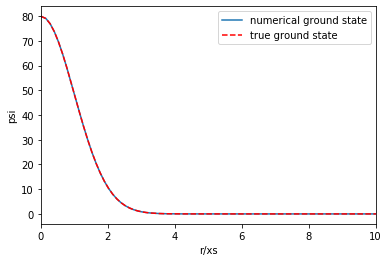
\includegraphics[width=0.8\linewidth]{gndstateQuasi2DHankel}
\caption{Comparison of the harmonic ground state and the numerical solution using the Quasi 2D Method}
\end{figure}


\section{Accuracy with no interactions}
In 3D, the ground state wavefunction with no interactions is shown below:

\begin{figure}[H]
\centering
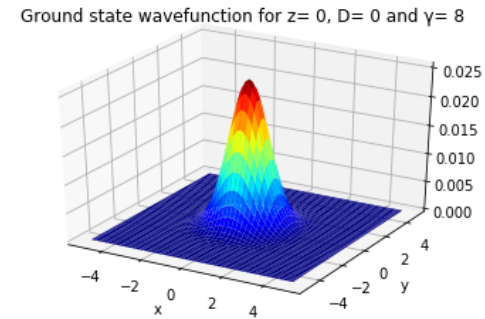
\includegraphics[width=0.8\linewidth]{gndstate1}
\caption{Ground state with $\gamma=8$}
\end{figure}

In 3D using a hankel transform and a cosine fast transform, we achieve the same ground state within $0.008\%$ of the true ground state with no interactions.

\begin{figure}[H]
\centering
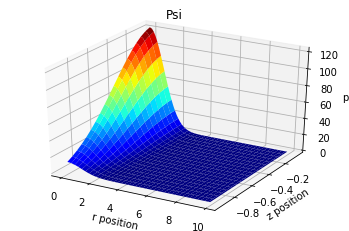
\includegraphics[width=0.8\linewidth]{gndstate3DHankel}
\caption{Ground state with $\gamma=5$ using the Hankel transform and cosine transform}
\end{figure}
	
Using the Hankel transform in 2D (1D computationally), we achieve very accurate results compared to the harmonic oscillator ground state.
\begin{figure}[H]
\centering
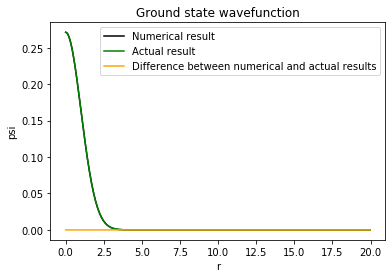
\includegraphics[width=\linewidth]{hankel 2d gnd state}
\caption{Ground state with 2D Hankel}
\end{figure}
We get an error of $\sim$0.0002\%.
Using the 2d fourier transform, we also achieve very accurate results.

\begin{figure}[H]
		\centering
		\begin{subfigure}[H]{0.49\linewidth}
			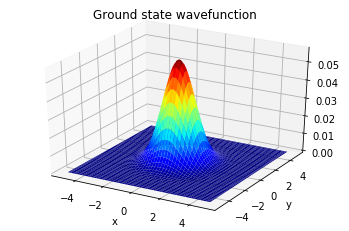
\includegraphics[width=\linewidth]{2d gnd state}
			\caption{Numerical 2D ground state wavefunction}
		\end{subfigure}
		\begin{subfigure}[h]{0.49\linewidth}
			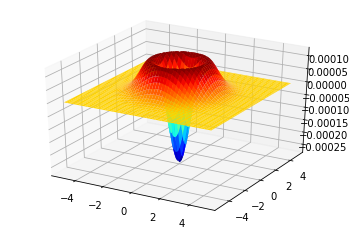
\includegraphics[width=\linewidth]{2d gnd state diff}
			\caption{Difference between numerical and actual solutions}
		\end{subfigure}
		\caption{2D Ground state using Fourier transforms (Sorry the graphs are small)}	
	\end{figure}
	
An average error of $\sim$0.2\% is achieved.


Lastly, at certain values of $\gamma$ and $D$, we expect the wavefunction have a bioconcave shape, like a red blood cell. This is shown clearly below.

\begin{figure}[H]
\centering
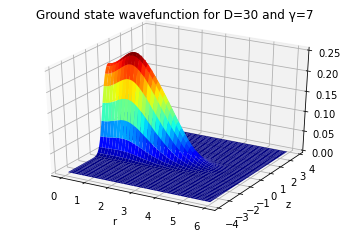
\includegraphics[width=\linewidth]{redbloodcell1}
\caption{3D plot of wavefunction using Hankel transform}
\end{figure}


\begin{figure}[H]
\centering
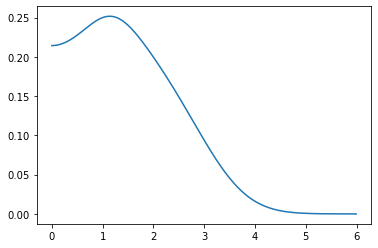
\includegraphics[width=0.8\linewidth]{redbloodcell2}
\caption{1D slice of the above wavefunction along z=0.}
\end{figure}


\section{Thomas Fermi}
The Thomas Fermi radius for a given axis is given by 
\begin{equation}
R_{i} = \sqrt{\frac{2\mu}{m\omega_{i}^2}},
\end{equation}
\begin{equation}
\mu = \frac{\hbar\bar{\omega}}{2}\bigg(\frac{Na}{x_{s}}\bigg)^{\frac{2}{5}},
\end{equation}
where $\omega_{i}$ is the harmonic frequency along that axis and $\mu$ is the chemical energy. 
DO CONTACT THOMAS FERMI DERIVATION AND THOMAS FERMI FROM QUASI 2D AND 1D PAPER

\section{Contact interactions}
A good check for validity is whether our solutions agree with the analytical solution in the Thomas-Fermi regime. Firstly, we compare our Quasi 2D solution with the analytical solution and we see we achieve very high accuracy.

 
\begin{figure}[H]
\centering
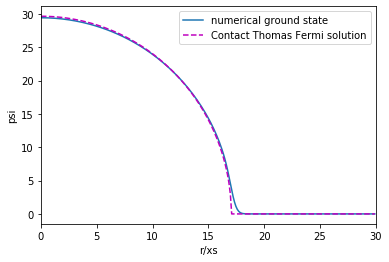
\includegraphics[width=0.8\linewidth]{ContactThomasFermiQuasi 2DHankelgamma=50No=4e5}
\caption{Thomas fermi regime with gamma = 50, N=4e5, using the Quasi 2D approach}
\end{figure}

We now compare our full 3D solution using the Hankel transform and the fast cosine transform, 

\begin{figure}[H]
\centering
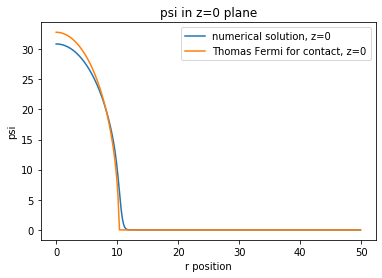
\includegraphics[width=0.8\linewidth]{Contact Thomas Fermi 3D Hankel gamma=5 No=2e5}
\caption{Thomas fermi regime with gamma = 5, N=2e5, using the 3D Hankel approach}
\end{figure}

The discrepancies between the analytical solutions and our solutions may be due to the fact that the Thomas-Fermi solution is only valid up to the edges of the cloud, where the Thomas-Fermi approximation becomes discontinuous.

\section{Purely dipolar interactions}
The extension of the Thomas-Fermi analysis remains valid in a purely dipolar condensate with modified terms, and when the Quasi 2D approximation becomes valid this becomes especially simple. This is because the dipolar interaction can be rewritten as a short-range term and a long-range one Ref\cite{Bao_2013}. This is shown below for dipoles orientated along the z-axis:

\begin{equation}
U_{3D} = \frac{1-3\cos^2(\theta)}{|\textbf{r}|^3} = -\frac{4\pi}{3}\delta(\textbf{r}) - \frac{\partial^2}{\partial z^2}\bigg(\frac{1}{|\textbf{r}|}\bigg)
\end{equation}

In the limit of large $D$ and $\gamma$ this long-range term can be neglected aswell as the kinetic energy term, thus resulting in the dipolar TF regime.


\begin{figure}[H]
\centering
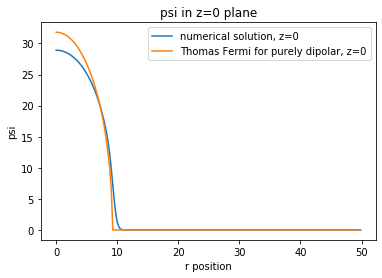
\includegraphics[width=0.8\linewidth]{Dipolar Thomas Fermi 3D Hankel gamma = 80 No=2e4}
\caption{Dipolar Thomas-fermi regime with gamma = 80, N=2e4, using the 3D Hankel approach}
\end{figure}

\begin{figure}[H]
\centering
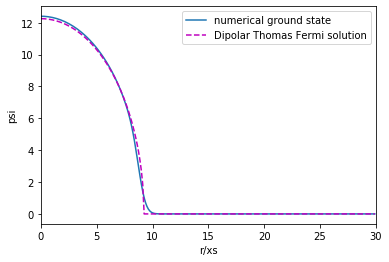
\includegraphics[width=0.8\linewidth]{Dipolar Thomas Fermi Quasi 2D Hankel gamma = 80 No = 2e4}
\caption{Dipolar-Thomas fermi regime with gamma = 5, N=2e5, using the Quasi 2D approach}
\end{figure}

\section{Discussion of stability of a purely dipolar gas}

\subsection{In a harmonic trap}

In general, the higher the trap ratio ($\lambda$), the more dipoles are required to make the condensate unstable. (This is due to fewer dipoles above or below any given dipole, since the dipole force is attractive in the cone above a dipole). Eventually, the BEC always becomes unstable for a large enough number of particles (for a given $C_{dd}$).

Figure 12 shows the stability using the 3D hankel approach. Black and white regions represent stable and unstable regimes respectively, and red represents the regime where biconcave (red blood cell) ground states are achieved. Figure 13 shows the same but using higher resolution, and unfortunately the colours are defined in the opposite way (obviously easily fixed). This shows strong agreement with fig[INSERT FIG NUMBER FROM RADIAL PAPER AND INSERT REFERENCE], showing the validity of our approach. 

\begin{figure}[H]
\centering
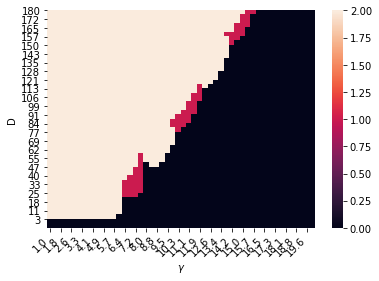
\includegraphics[width=\linewidth]{stableplot1}
\caption{Stability plot of gamma against the dimensionless parameter D. The x axis is dipole strength and the y axis is gamma.}
\end{figure}

\begin{figure}[H]
\centering
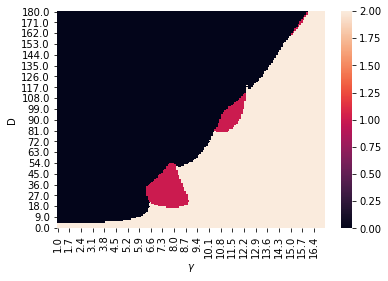
\includegraphics[width=\linewidth]{best harmonic stability plot}
\caption{Stability plot of gamma against the dimensionless parameter D. The x axis is dipole strength and the y axis is gamma.}
\end{figure}

\subsection{In a pancake trap}

 In a similar fashion to the harmonic trap, we define the dimensionless dipole interaction parameter, \scalebox{1.2}{$D^{box} =  \frac{m N \mu_0 \bar{\mu}^2}{4\pi \hbar^2 L}$} where $L$ is the length scale of the trap, normally defined to be the size of the trap in the r direction.
We see that $\gamma$ and $D$ are different, and using equation \eqref{Vextbox}, $\gamma$ is now \scalebox{1.2}{$\frac{mw_z L^2}{\hbar}$}. Note now $\gamma \propto w_z$. 
To give an idea of the ranges of $\gamma$ and $D$, we use a typical set of parameters shown below:
\begin{align*}
m=2.78\times10^{-25}[kg], w_z=20\pi-100\pi[rad/s], \\ L=1\times10^{-5}[m], N=10^5, \bar{\mu}\approx 7\mu_B [J/T]
\end{align*}
where $\mu_B$ is the Bohr magneton.

We get $\gamma = 16-82$ and $D_{box}=104$.

However these numbers greatly depend on $L$, which is proportional to the trap size. 
Defining $\gamma$ in this way is completely analogous to the harmonic case, as for both cases we define it as 
\begin{equation}
\gamma = \frac{L^{2}}{l_{z}^{2}}.
\end{equation}
where L and $l_{z}$ are the length scales in the r and z direction respectively (\scalebox{1.1}{$l_{z} = \sqrt{\frac{\hbar}{m\omega_{z}}}$}). However, these don't equate to the same geometric situations as L represents a different fraction of the cloud size if it's defined to be the size of the trap. This means  the ranges of gamma for the two cases which equate to roughly the same geometric ratios will be different. To get round this, we can define the box potential length scale to be a fraction of the box size, so when $\gamma =1$ the height and width of the cloud will be approximately equal. This means that the ranges of gammas will equate to the same geometric ratios with this adjustment. 
Going into dimensionless units and setting the size of the box to be $3L$, we achieve the following graph.

\begin{figure}[H]
\centering
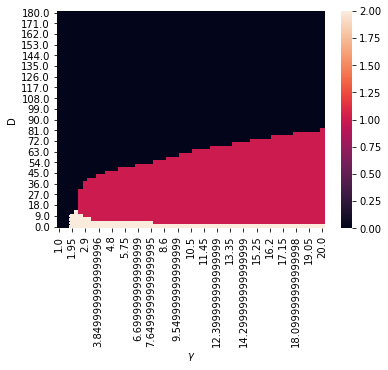
\includegraphics[width=\linewidth]{box potential stability plot gamma = 10}
\caption{Stability plot of gamma against the dimensionless parameter D, with the size of the trap set to $3L$. White regions show stable areas. Red regions show stable areas, but with the maximum value of the wavefunction not at the centre. Black regions indicate instability.}
\end{figure}

This diagram shows for low D the maximum density still lies in the middle (show as white in the diagram), which is expected for D=0. As both D and gamma increase the maximum density lies at the outer regions of the cloud. This density oscillation is shown in Figure 15 [NEED TO INCLUDE THE VALUE OF D AND GAMMA FOR THIS PLOT]. 
\begin{figure}[H]
\centering
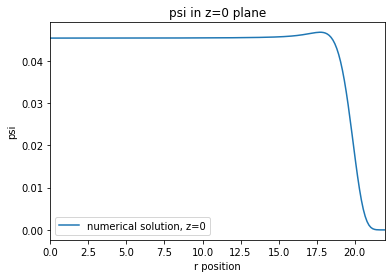
\includegraphics[width=\linewidth]{density oscillation}
\caption{psi in the z=0 plane using a circular box potential, the maximum density is situated close to the edge of the cloud, where in this case $R_{box}=20L$.}
\end{figure}

In [INSERT REFERENCE FOR NU PAPER] they predict for a gas unconfined in the r plane and harmonically confined in the z direction, that
\begin{equation}
\gamma\propto D^{2}
\end{equation} 
on the stability boundary for a purely dipolar gas. This is shown from fig 5(b) IN REF [INSERT REFERENCE FOR NU PAPER] where it can be seen that for $g_{s} =0$,
\begin{equation}
 \nu_{d}=const.
\end{equation}
From this (10.2) can be derived. It follows from this that as the size of our box increases, it would seem sensible for our stability plot to tend to (10.2). Figure 14 seems to show that this might be true for high gamma, but a more conclusive plot is definitely needed. There seems to be the opposite relationship for lower gamma, as can be shown by figure 16 which used \scalebox{1.1}{$R_{box}=20L$}, but this may just be a problem with the code. Over the next week or so we should be able to get some better plots, these are really just giving a rough idea of what it looks like.

\begin{figure}[H]
\centering
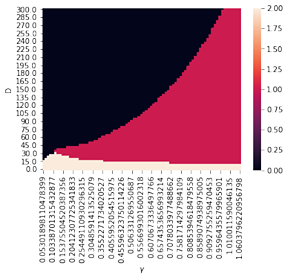
\includegraphics[width=\linewidth]{stablebox1}
\caption{Stability plot of gamma against the dimensionless parameter D, with \scalebox{1.1}{$R_{box}=20L$}. White regions show stable areas. Red regions show stable areas, but with the maximum value of the wavefunction not at the centre. Black regions indicate instability.}
\end{figure}

\section{Stability outside the purely dipolar regime}
We can also analyse the stability of the gas outside the purely dipolar regime. In [INSERT REFERENCE FOR NU PAPER] they determine two dimensionless parameters ${\nu,\nu_{d}}$, where if constant, the GPE is invariant. For our analysis we confine the dipoles to be aligned in the z direction which leads to the following,
 \begin{equation}
\nu = \frac{n[3g+2C_{dd}]}{3\hbar\omega_{z}l_{z}}
\end{equation} 
\begin{equation}
\nu_{d} = \frac{nC_{dd}}{3\hbar\omega_{z}l_{z}}
\end{equation} 
These are equavalent to equations (6) and (16) respectively in [INSERT REFERENCE FOR NU PAPER] with $\alpha=0$.
Rewriting them in terms of our dimensionless variables, we get the following expressions:

 \begin{equation}
\nu = \frac{(3g_{s}+8\pi D)l_{z}}{3\pi L}
\end{equation} 
\begin{equation}
\nu_{d} = \frac{4Dl_{z}}{3L}
\end{equation} 
For $\gamma=100$ we achieve good agreement with the unconfined case.

\begin{figure}[H]
\centering
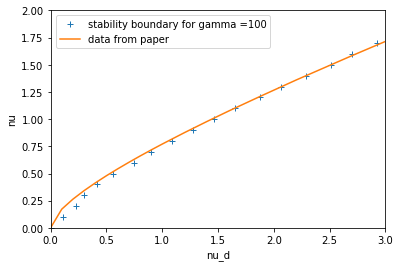
\includegraphics[width=\linewidth]{stability boundary comparison}
\caption{stability boundary, where for any $\nu_{d}$ above the boundary, the BEC becomes unstable. We see our results are in good agreement with the unconfined case.}
\end{figure}

For $\gamma=10$, the stability boundary starts to deviate from the unconfined case and it seems it increase in stability for a given \scalebox{1.1}{$\nu$}. Again, this is only a rough idea of what happens as $\gamma$ decreases, hopefully we will have more conclusive plots by the end of the week.

\begin{figure}[H]
\centering
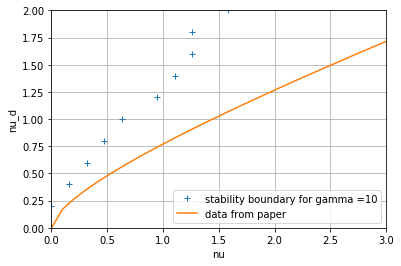
\includegraphics[width=\linewidth]{stability boundary gamma=10}
\caption{We see that the stability boundary may be higher for a lower gamma, when the unconfined approximation is no longer valid.}
\end{figure}

\section{Issues}
One issue we seem to be getting is that the code doesn't work for very high $\gamma$. One reason is my idea that the time scale was independent of $\gamma$ may be incorrect, as by dividing dt by $\gamma$ seems to give more sensible results at very high $\gamma$. However this does increase computational time due to more iterations being needed for convergence with low dt. But even accounting for this, there still seems to be issues for very high $\gamma$. My guess at the moment is a floating point precision error, as for some calculations we are using variables that are proportional to $\gamma^{2}$ along with variables that are not. This may lead to a loss of information. This is the main justification for having the length scale be a fraction of the box size rather than the box size itself, as lower gammas are needed to achieve the same geometric situations. It seems strange that a precision error would lead to large differences, but I can't see any other reason for this and the code clearly works very well for sensible ranges of $\gamma$. 

 \end{multicols}


\bibliographystyle{unsrt}
\bibliography{references}


\end{document}